\chapter{SAMBA 3}
Este capítulo descreve os procedimentos necessários para a instalação e a configuração do Samba 3 para trabalhar como controlador de domínio, servidor de impressão e servidor de arquivos, respeitando as regras de usuários e permissões.
Primeiramente explicará todo o processo de instalação do Samba 3, algumas formas de alterar o arquivo de configuração e como iniciar os serviços do mesmo. Posteriormente mostrará o passo-a-passo de como se deve configurar o Samba 3 para trabalhar como um domínio, criação dos que irão logar usuários no domínio, explicação das variáveis que podem ser usadas na criação de um compartilhamento de arquivos, para definirem segurança de acesso aos arquivos, compartilhar impressoras na rede, e por fim a explicação do procedimento para a inserção de máquinas Windows e Linux no domínio.

\section{Instalação do Samba 3}

O pacote Samba 3 pode ser instalado através do repositório de sistemas da distribuição Linux na qual será configurado (neste trabalho foram utilizadas as distribuições Ubuntu 11.04 e Debian 6.0.5). Antes da instalação é necessário atualizar a base de dados do repositório para que possa instalar a versão mais atual do Samba 3.

Duas observações devem ser feitas. Na primeira, todos os comandos precedidos do síbolo ``#'' necessítam de permissões de root para serem executados, e na segunda, que todos os comandos de instalação que não informarem repositório específico, possuem suporte nas distribuições Ubuntu e Debian.
 
\begin{enumerate}
    \item \textbf{\# apt-get update} - Atualiza a base de dados do repositório no Ubuntu.
    \item \textbf{\# apt-get install samba} - Realiza a instalação do pacote Samba 3.
    \item \textbf{\# apt-get install smbclient} - Pacote que mostra as informações do servidor Samba 3 e permite acesso de compartilhamentos no Windows ou Linux a partir de uma máquina Linux.
\end{enumerate}

\section{SWAT - Gerenciando o Samba 3 pelo browser}

O SWAT é uma ferramenta para a edição do /etc/smb.conf, porém por meio de uma interface gráfica. Com ele é possível compartilhar impressoras, arquivos, criar usuários, permitir ou restringir acessos.

\begin{enumerate}
 \item \textbf{\# apt-get install swat} - Instala a ferramenta gráfica SWAT para o gerenciamento do Samba 3.
    \item \textbf{\$ firefox localhost:901} - Endereço de acesso no \textit{browser} (neste caso o Firefox) para acessar o SWAT.
\end{enumerate}

Ao acessar o SWAT pelo navegador, o usuário deve informar o usuário root e sua senha para ter acesso total aos controles do SWAT. Se for realizado acesso com um usuário diferente, a visão dos controles do SWAT mudará de acordo com as permissões desse usuário no sistema. Após o login no sistema, pode-se observar na barra de ferramentas as opções de configuração do SWAT, conforme Figura \ref{swat}. A função de cada opção é detalhada a seguir:

\begin{figure}[ht]
   	\centering
    \scalebox{1}{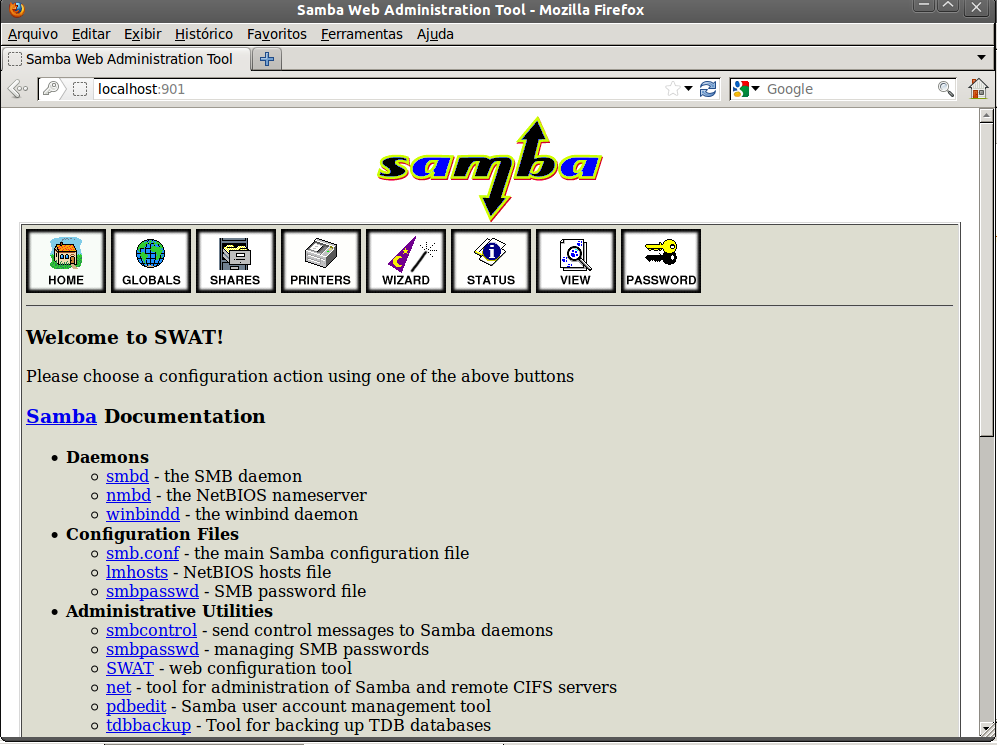
\includegraphics{figuras/swat}}
   	\caption{Tela do SWAT}
    \label{swat}
\end{figure}

\begin{itemize}
    \item \textbf{Home} - Documentação do Samba 3
    \item \textbf{Globals} - Variáveis globais de configuração do Samba 3
    \item \textbf{Shares} - Ativar compartilhamentos de diretórios e arquivos
    \item \textbf{Printers} - Compartilhamento de impressoras
    \item \textbf{Wizard} - Escreve as modificações no arquivo smb.conf do Samba 3
    \item \textbf{Status} - Status do servidor com usuário, compartilhamento dos ativos e arquivos abertos
    \item \textbf{View} - Mostra o arquivo smb.conf
    \item \textbf{Password} - Cadastrar o usuário, máquinas e mudar senha dos usuários no servidor
\end{itemize}

Por se tratar de uma ferramenta gráfica o SWAT torna mais fácil a edição e adição de configurações no smb.conf, mas toda vez que as configurações são alteradas e salvas ele gera um novo arquivo smb.conf e com isso apaga todos os possíveis comentários existentes no arquivo. Por se tratar de um arquivo com muitas variáveis, parâmetros e seções, nesse trabalho o foco será a edição através de editores de texto padrão como o Vim, pois assim algumas configurações podem ser inseridas como comentários para fins de explicação ou como base para futuras modificações.

\section{Iniciando Samba 3}

Com todos os componentes instalados a aplicação pode ser iniciada. O Samba 3 trabalha com dois \textit{daemon} principais, geralmente eles se encontram no /usr/sbin/,  que são: SMBD e o NMBD

O SMBD permite compartilhamento de arquivos e impressoras em uma rede SMB e provê autorização e autenticação a usuários SMB. O NMBD cuida do \textit{Windows Internet Name Service} (WINS) e auxilia com a navegação e resolução de nomes.\cite{SAMBA}

Para iniciar os processos do Samba 3, utiliza-se o seguinte comando:
\begin{itemize}
	\item \textbf{\# /etc/init.d/smbd start} - Inicia o Samba 3.	
\end{itemize}

Por ter sido instalado em um sistema operacional Linux, o Samba 3 pode conter varias formas de iniciar e de parar, dependendo da distribuição na qual ele foi instalado.

Ubuntu:
\begin{itemize}
	\item \textbf{\# service smbd start} - Inicia o Samba 3.
	\item \textbf{\# service smbd stop} - Para o processo do Samba 3.
	\item \textbf{\# service smbd restart} - Finaliza o processo existente e cria outro para o Samba 3.
	\item \textbf{\# /etc/init.d/smbd start} - Para iniciar o Samba 3 em computadores com Debian 6.
	\item \textbf{\# /etc/init.d/smbd stop} - Para o Samba 3 no Debian 6.
	\item \textbf{\# /etc/init.d/smbd restart} - Finaliza o processo existente e cria outro para o Samba 3.
\end{itemize}

Debian:
\begin{itemize}
	\item \textbf{\# service samba start} - Inicia o Samba 3.
	\item \textbf{\# service samba stop} - Para o processo do Samba 3.
	\item \textbf{\# service samba restart} - Finaliza o processo existente e cria outro para o Samba 3.
	\item \textbf{\# /etc/init.d/samba start} - Para iniciar o Samba 3 em computadores com Debian 6.
	\item \textbf{\# /etc/init.d/samba stop} - Para o Samba 3 no Debian 6.
	\item \textbf{\# /etc/init.d/samba restart} - Finaliza o processo existente e cria outro para o Samba 3.
\end{itemize}

\section{Seções}

No Samba 3, as configurações de compartilhamentos, impressoras e gerais, são realizadas através de um único arquivo de configuração, o ``/etc/samba/smb.conf". Esse arquivo para melhor organização, fica dividido em sessões, sendo a primeira sessão nomeada como [global], onde são definidas as configurações gerais do servidor. Também podem ser criadas sessões adicionais para cada compartilhamento, sendo nomeadas com o nome do mesmo. Se for necessário criar um compartilhamento com o nome ``arquivo", a sessão que deve ser criada no arquivo de configuração deve ser [arquivo].

\section{Variáveis de substituição do Samba 3}

Existem variáveis especiais que podem ser usadas no arquivo de configuração do Samba 3 e são substituídas por parâmetros especiais no momento da conexão do usuário \cite{FOCA}. Um exemplo de utilização de variáveis de substituição seria mudar a localização do diretório home do usuário conforme no Quadro \ref{variavel_home}:\\

\begin{lstlisting}[caption=Exemplo de utilização das variáveis de substituição,label={variavel_home}]	
[home]
	
comment = Diretorio home do usuario

path = /home/usuarios/%u
\end{lstlisting}          

Ao longo deste trabalho diversas variáveis de substituição serão utilizadas, principalmente nos scripts aqui propostos. Cada uma das variáveis são descritas em detalhes a seguir:

\%S - O nome do serviço atual, se existir. Seu uso é interessante, principalmente no uso de diretórios homes.

\%P - O diretório raíz do serviço atual, se existir.

\%u - O nome de usuário do serviço atual, se aplicável. Esta variável é bastante útil para programação de scripts e também para criar arquivos de log personalizados, etc.

\%g - O grupo primário do usuário \%u.

\%U - O nome de usuário da seção (o nome de usuário solicitado pelo cliente, não é uma regra que ele será sempre o mesmo que ele recebeu).

\%G - O nome do grupo primário de \%U.

\%H - O diretório home do usuário, de acordo com \%u.

\%v - A versão do Samba.

\%h - O nome DNS da máquina que está executando o Samba.

\%m - O nome NetBIOS da máquina do cliente. Isto é muito útil para log de conexões personalizados e outras coisas úteis.

\%L - O nome NetBIOS do servidor. Como o servidor pode usar mais de um nome no Samba (aliases), você poderá saber com qual nome o seu servidor está sendo acessado e possivelmente torna-lo o nome primário de sua máquina.

\%M - O nome DNS da máquina cliente.

\%N - O nome do seu servidor de diretórios home NIS. Este parâmetro é obtido de uma entrada no seu arquivo auto.map. Se não tiver compilado o SAMBA com a opção --with-automount então este valor será o mesmo de %L.

\%p - O caminho do diretório home do serviço, obtido de uma entrada mapeada no arquivo auto.map do NIS. A entrada NIS do arquivo auto.map é dividida na forma ``\%N:\%p".

\%R - O nível de protocolo selecionado após a negociação. O valor retornado pode ser CORE, COREPLUS, LANMAN1, LANMAN2 ou NT1.

\%d - A identificação de processo do processo atual do servidor.

\%a - A arquitetura da máquina remota. Somente algumas são reconhecidas e a resposta pode não ser totalmente confiável. O Samba atualmente reconhece Samba, Windows for Workgroups, Windows 95, Windows NT e Windows 2000. Qualquer outra coisa será mostrado como \textit{``UNKNOWN"} (desconhecido).

\%I - O endereço IP da máquina do cliente.

\%T - A data e hora atual.

\%\$(var\_ambiente) - Retorna o valor da variável de ambiente especificada.

\section{Configuração do Samba para ser um PDC}

O arquivo de configuração se encontra no diretório /etc, onde está a maioria dos arquivos de configuração dos programas no Linux. Para realizar as configurações, siga as etapas que serão explicadas.

Por se tratar de um arquivo de configuração mutável uma boa prática é a utilização de backups dos arquivos originais, pois caso o sistema pare de funcionar devido a uma má configuração ou seja necessário para leitura posterior, o administrador de rede terá uma copia de segurança.

\begin{enumerate}
	\item \textbf{\# cp /etc/samba/smb.conf /etc/samba/smb.conf.bkp} - Por motivo de segurança é recomendado fazer um backup do arquivo. Ele contém exemplos comentados das possíveis configurações do Samba 3, auxiliando o profissional de TI no momento de sua configuração.
\end{enumerate}

O arquivo original do Samba 3 vem repleto de comentários de possíveis variáveis que podem ser utilizadas ou contém algum tipo explicação. Para a leitura do administrador os comentários complicam pois muitas informações não são necessárias dependendo da configuração e uma maneira de melhorar é a remoção dos comentários.

\begin{enumerate}
	\item \textbf{\# testparm -s /etc/samba/smb.conf.bkp $>$ /etc/samba/smb.conf} - Removerá os comentário para melhor leitura do arquivo. Observação: o arquivo de origem não pode ser o smb.conf pois ele irá se rescrever e o arquivo só conterá a seção [global] vazia.
\end{enumerate}

Para editar as configurações e definir as funções que serão providas pelo Samba 3, pode-se utilizar qualquer comando ou aplicativo para edição de texto. 

\begin{enumerate}
	\item \textbf{\# vim /etc/samba/smb.conf} - Para editar o arquivo e adicionar as seções, parâmetros e variáveis.
\end{enumerate}

Agora é necessário inserir, modificar e remover alguns parâmetros na seção [global] para que o Samba 3 se comporte como um PDC. Conforme o Quadro \ref{smb_global}\\

\begin{lstlisting}[caption=Variáveis para que o Samba 3 funcione como PDC,label={smb_global}]
[global] 

workgroup = IFF.BOMJESUS

server string = Compartilhamento de Arquivos do IFF - Campus Bom Jesus do Itabapoana

security = user

netbios name = battousai-share	

domain master = yes

domain logons = yes

enable privileges = yes

passdb backend = tdbsam
	
encrypt passwords = true

preferred master = yes

local master = yes

os level = 100

map to guest = Bad User

panic action = /usr/share/samba/panic-action \%d	
\end{lstlisting}

Explicação das variáveis utilizadas:

\begin{itemize}
	\item \textbf{workgroup} - Nome do servidor de domínio.
	\item \textbf{server string} - Descrição do servidor que aparece na barra de título das janelas do compartilhamento.
	\item \textbf{security} - Tipo de segurança do compartilhamento. Existem os tipos domain, user e share.
		\begin{enumerate}
			\item {share}  - É utilizado quando o compartilhamento será aberto, onde todos os usuários conectados serão guest e sem a necessidade de realizar login.
			\item {user} - Todos os usuários que tentarem se conectar terão que se identificar por meio de um login e uma senha.
			\item {domain} - Quando um servidor de domínio será responsável pela identificação e segurança dos usuários.
		\end{enumerate} 
	\item \textbf{netbios name} - Nome da netbios do servidor.
	\item \textbf{encrypt passwords} - Quando informado o valor ``true" as senhas informadas para o servidor serão criptografadas.
	\item \textbf{domain master} - Informa que o servidor Samba 3 será o domínio principal da rede.
	\item \textbf{domain logons} - O servidor Samba 3 passa a ser um controlador de domínio.
	\item \textbf{enable privileges} - Habilita alguns privilégios no Samba 3. Alguns deles:
		\begin{enumerate}
			\item {SeAddUsersPrivilege} - Adicionar usuários e grupos no domínio 
			\item {SeDiskOperatorPrivilege} - Gerencia os discos compartilhados 
			\item {SeMachineAccountPrivilege} - Adicionar maquinas no domínio 
			\item {SePrintOperatorPrivilege} - Gerencia as impressoras
		\end{enumerate}
	\item \textbf{passdb backend} - Aceita valores smbpasswd ou tdbsam . Define qual será a forma de armazenagem dos registros dos usuários.
	O tdbsam oferece duas vantagens sobre o smbpasswd: oferece um melhor desempenho em servidores com um grande número de usuários cadastrados e oferece suporte ao armazenamento dos controles SAM (\textit{Software Asset Management}) estendidos usados pelas versões server do Windows. O uso do tdbsam é fortemente recomendável caso seu servidor tenha mais do que algumas dezenas de usuários cadastrados ou caso você pretenda usar seu servidor Samba como PDC da rede. Ele é também um pré-requisito caso você precise migrar um domínio NT já existente para o servidor Samba. \cite{BACKEND}
		\begin{enumerate}
			\item{smbpasswd} - O smbpasswd é o backend mais simples. Nele, as senhas são salvas no arquivo ``/etc/samba/smbpasswd" e são transmitidas de forma encriptada através da rede, com suporte ao sistema NTLM, usado pelas versões contemporâneas do Windows. A vantagem do smbpasswd é que ele é um sistema bastante simples. Embora encriptadas, as senhas são armazenadas em um arquivo de texto, com uma conta por linha.\cite{BACKEND}
			\item{tdbsam} - O tdbsam usa uma base de dados muito mais robusta, armazenada no arquivo ``/var/lib/samba/passdb.tdb".\cite{BACKEND}
		\end{enumerate}
	\item \textbf{local master} - Define se o servidor será o \textit{Master Browser}.
	\item \textbf{os level} - Valor que será passado na eleição para definir o mestre da rede. O valor máximo é 100, assim vencendo os valores padrões de ``os level" o servidores Windows.
%	\item \textbf{win support} - Se nmbd será um servidor WINS.
	\item \textbf{map to guest} - Torna usuário guest todos que não conseguirem se identificar com um login e senha valida.
	\item \textbf{panic action} - Comando que será executado caso o smbd ou nmbd parem de funcionar.
\end{itemize}

Com todas as variáveis devidamente adicionadas o servidor Samba 3 precisa ser reiniciado para que todas as modificações entrem em vigor.

\begin{enumerate}
	\item \textbf{\# testparm} - Verifica se existe algum erro de sintaxe no arquivos de configuração no smb.conf. Exemplo de execução que pode ser visto na Figura \ref{testparm}
	\item \textbf{\# /etc/init.d/smbd restart} - Reinicia o Samba 3.
	\item \textbf{\# /etc/init.d/nmbd restart} - Reinicia o servidor de nomes do Samba 3.
\end{enumerate}

\begin{figure}[ht]
   	\centering
    \scalebox{1}{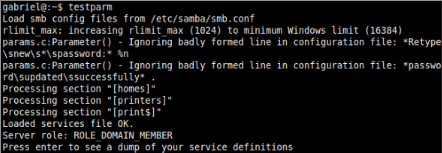
\includegraphics{figuras/testparm}}
   	\caption{Saída do testparm}
    \label{testparm}
\end{figure}

\section{Cadastro de Usuário}

Os usuários que terão acesso e permissões de login no domínio devem ser criados no servidor Linux, onde se encontra o Samba 3. O usuário root tem que ser cadastrado no Samba 3 antes de qualquer outro usuário, pois ele é o administrador da aplicação.

\begin{itemize}
	\item \textbf {\# smbpasswd -a root} - Uma senha terá que ser informada e precisa ser a mesma do usuário no sistema.
\end{itemize}

Cada usuário no sistema deverá conter uma pasta com o nome de ``profile.pds". Essa pasta irá conter informações das sessões de \textit{logon} que o usuário fez no servidor de domínio. Para automatizar a criação dessa pasta no diretório \textit{home} dos usuários, cria-se o diretório no /etc/skel.

\begin{itemize}
	\item \textbf{\# mkdir /etc/skel/profile.pds} - O /etc/skel armazena todos os diretórios e arquivos que serão criados juntos com o usuário no sistema.
\end{itemize}

Antes de cadastrar os usuários no Samba 3 eles precisam ser criados no sistema.

\begin{itemize}
	\item \textbf{\# adduser "--disabled-login usuario} - Comando para a criação mais completa de usuário no Linux com nome completo, telefone e outros dados, porém sem a permissão de login e entre outros dados.
\end{itemize}

Após o usuário ser criado no sistema, ele necessita ser cadastrado no Samba 3.

\begin{itemize}
	\item \textbf{\# smbpasswd -a usuario} - Informe a mesma senha cadastrada no Linux.
\end{itemize}

\section{Cadastro de Máquinas}

Da mesma forma que os usuário têm que ser cadastrados no sistema, as máquinas que poderão entrar no domínio também devem ser cadastradas. As máquinas são cadastradas como usuários normais no Linux antes de serem cadastradas no Samba 3, porém sem pasta home e sem bash para login.

\begin{enumerate}
	\item \textbf{\# groupadd machine} - Cria o grupo no qual serão adicionadas as máquinas cadastradas para melhor organização dos usuários no Linux.
	\item \textbf{\# useradd "--home /dev/null "--shell /bin/false "--disabled-login "--group machine computador1\$} - 	Comando para a criação da máquina no sistema Linux. Por padrão se adiciona o \$ no final do nome pois é dessa forma que o Samba 3 irá identificar que o usuário na verdade é uma máquina. 
	\item \textbf{\# passwd -l computador1\$} - Desativa a mudança da senha para o usuário/máquina.
\end{enumerate}

Após a criação do usuário/máquina no sistema agora ele tem que ser cadastrado no Samba 3.

\begin{itemize}	
	\item \textbf{\# smbpasswd -a -m computador1\$} - Cadastra a máquina no Samba 3.
\end{itemize}


\section{Script de Cadastro de Usuários e Máquinas}

Para facilitar a criação e exclusão dos usuários no sistema e no Samba 3, foi feito o script \textbf{smbmanager.sh}\footnote[1]{Pode ser baixado em https://github.com/GabrielRocha/Monografia/blob/master/latex/Scripts/smbmanager.sh} conforme o anexo no Apêndice A1. Com ele é possível criar usuários e máquinas, adicionar usuários em grupos e também excluí-los do sistema.

O script tem que ter a permissão de root para que possa ser iniciado.

\begin{enumerate}
	\item \textbf{\# chmod +x smbmanger.sh} - Adiciona a permissão de execução ao script.
	\item \textbf{\# cp smbmanager.sh /usr/sbin/} - Transferindo o script para a pasta /usr/sbin/ o script poderá ser iniciado em qualquer caminho que o usuário esteja.
	\item \textbf{\# ./smbmanager.sh} - Execução do \textit{script}. Figura \ref{smbmanager}
\end{enumerate}

\begin{figure}[ht]
   	\centering
    \scalebox{1}{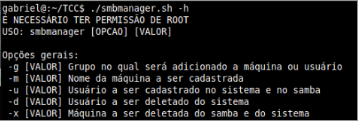
\includegraphics{figuras/smbmanager}}
   	\caption{Saída do smbmanager}
    \label{smbmanager}
\end{figure}

\section{Migração dos Usuários Administradores e Users do Linux para o Windows}

Para que o Windows possa reconhecer um grupo de usuários administradores do Linux como Power Users e Domain Users deve se mapear os grupos pelo RID dos mesmos. A Tabela \ref{tab} apresenta alguns dos grupos e seus respectivos RID (\textit{Relative Identifier}). Os comandos a seguir devem ser utilizados para mapear esses grupos no Samba 3.

\begin{table}[h!]
	\centering
	\caption{Tabela do RID (\textit{Relative Identifier}) Windows \cite{RID}}
	\begin{tabular}{cccc}
		
		\hline
		
		Well-Known Entity & RID & Type &	Essential \\
		
		\hline
		
		\hline
		
		Domain Administrator & 500 & User & No \\
		Domain Guest & 501 & User & No \\		
		Domain KRBTGT & 502	& User & No \\
		Domain Admins & 512 & Group & Yes \\
		Domain Users & 513 & Group & Yes \\
		Domain Guests & 514 & Group & Yes \\
		Domain Computers & 515 & Group & No \\
		Domain Controllers & 516 & Group & No \\
		Domain Certificate Admins & 517 & Group & No \\
		Domain Schema Admins & 518 & Group & No \\		
		Domain Enterprise Admins & 519 & Group & No \\
		Domain Policy Admins & 520 & Group & No \\
		Builtin Admins & 544 & Alias & No \\
		Builtin users & 545 & Alias & No \\
		Builtin Guests & 546 & Alias & No \\
		Builtin Power Users & 547 & Alias & No \\
		Builtin Account Operators & 548 & Alias & No \\
		Builtin System Operators & 549 & Alias & No \\
		Builtin Print Operators	& 550 & Alias & No \\
		Builtin Backup Operators & 551 & Alias & No \\
		Builtin Replicator & 552 & Alias & No \\
		%Builtin RAS Servers & 553 & Alias & No \\
		 	
		\hline
	\end{tabular}
	\label{tab}
\end{table}

\clearpage

\begin{itemize}
	\item \textbf{\# net groupmap list} - Liste os grupos existentes mapeados, caso não tenha o grupo siga os passos a seguir.
\end{itemize}
\begin{enumerate}
	\item \textbf{\# net groupmap add ntgroup=`Domain Admins' rid=512 unixgroup=admin} - Irá mapear o grupo admin para o grupo Domain Admins do Windows.
	\item \textbf{\# net groupmap add ntgroup=`Domain Users' rid=513 unixgroup=users} - Mapea o grupo users com o Domain Users do Windows.
\end{enumerate}

\begin{enumerate}
	\item \textbf{\# net groupmap delete ntgroup=`Domain Admins'} - Caso queira remover um mapeamento de grupo.
	\item \textbf{\# net groupmap modify ntgroup=`Domain Admins' rid=512 unixgroup=admin} - Caso tenha necessidade de modificar um mapeamento.
\end{enumerate}

Dessa forma, se o usuário logar com os usuários que estejam no grupo admin em algum terminal Windows no domínio, ele terá permissões de administrador.

\section{Perfis Móveis}

Para que as configurações e personalizações do perfil do usuário no Windows sejam salvas é necessário a criação de um perfil móvel no servidor Samba 3. 
A vantagem de se utilizar um perfil móvel é que não existe a obrigatoriedade de se realizar backup na máquina do usuário, pois os arquivos são salvos no servidor, sendo assim é só o usuário fazer o login em outra máquina Windows que o seu perfil e os seus dados serão migrados para o novo computador. Porém o perfil móvel tem um problema que é a quantidade de dados armazenados. Se o número de usuários e dados de cada um for muito grande, cria-se a necessidade de ter um servidor com muito espaço de armazenamento e uma rede muito bem estruturada. 

Para ativar a configuração de perfil móvel no Samba 3 deve-se adicionar no [global] as variáveis mostradas no Quadro \ref{logon_path} \\

\begin{lstlisting}[caption=Variáveis necessárias para o perfil móvel,label={logon_path}]	
logon path = \\%L\Profiles\%U

logon home = \\%L\Profiles\%U

logon drive = H:	
\end{lstlisting}


\begin{enumerate}
	\item \textbf{logon path} - Serve para indicar o caminho onde vão ficar os perfis no Windows XP/Vista/7 
	\item \textbf{logon home} - Indica o caminho para os perfis em versões mais antigas do Windows, como 95/98.
	\item \textbf{logon drive} -  Unidade que será mapeada com o caminho $\backslash$$\backslash$servidor$\backslash$profiles$\backslash$"nome do usuário" no Windows.
\end{enumerate}

No exemplo apresentado, o diretório profile criado fica compartilhado para que seja mapeado na unidade H do usuário no Windows.

Após a definição dessas três opções na seção [global], deve-se criar uma seção [profiles] contendo alguns comandos que serão detalhados a seguir no Quadro \ref{smb_profile}.\\

\begin{lstlisting}[caption=Variáveis para criação do compartilhamento profile,label={smb_profile}]	
[profiles] 

path = /var/samba/%U 
	
writeable = yes 
	
browseable = no 
	
create mask = 0600 
	
directory mask = 0700 
	
available = yes
	
\end{lstlisting}

\begin{itemize}
	\item \textbf {path} - Caminho da pasta que vai ser compartilhada.
	\item \textbf {writeable} - Permite a escrita no diretório e nos arquivos.
	\item \textbf {browseable} - Define se o compartilhamento poderá ser visto na pasta principal do compartilhamento ou somente pelo endereço completo.
	\item \textbf {create mask} - Força a criação dos arquivos com a permissão 0600, assim somente os donos do arquivo poderão alterar os arquivos.
	\item \textbf {directory mask} - Criação dos diretórios com permissão 0700.
	\item \textbf{available} - (Yes/No) Se o compartilhamento estará acessível ou não no servidor.
\end{itemize}

\section{Compartilhamento de Arquivos}

O compartilhamento de arquivos é dado pela adição de seções no arquivo smb.conf. Como pode ser visto no Quadro \ref{smb_diretoria}\\

\begin{lstlisting}[caption=Criação de uma seção para compartilhamento de arquivos,label={smb_diretoria}]
[Diretoria]

path = /media/diretoria

read only = no

valid users = +diretoria

force group = diretoria

create mask = 0770

directory mask = 0770

browseable = no
	
\end{lstlisting}

\begin{itemize}
	\item \textbf{[Diretoria]} - Nome do compartilhamento que será mostrado no servidor.
	\item \textbf{path} - Nele devemos mapear diretórios que serão compartilhados na rede. 
\end{itemize}

	Cabe ressaltar que após a criação desses diretórios, é necessário o ajuste das permissões de acesso, do dono do diretório e do grupo do diretório, utilizando os programas chmod e chown, respectivamente. O ajuste varia caso a caso, e deve ser realizado com cautela, para não dar mais permissões que o necessário. Uma breve explicação sobre o chmod e chown é realizada a seguir:

\# chmod - Define as permissões do arquivo. Exemplo: \# chmod 774 -R /pasta\_criada - essas permissões definem que o usuário proprietário do diretório e todos os usuário do grupo do diretório terão controle total no diretório e em seus arquivos e que os outro usuário poderão apenas listar os arquivos que se encontram no diretório.

\# chown - Define qual será o usuário e grupo proprietário do diretório ou arquivo. Exemplo: \# chown usuario.grupo /diretorio .

\begin{itemize}
	\item \textbf{read only} - Define se o compartilhamento estará com permissão de somente leitura ou não.
	\item \textbf{Valid users} - Define quais usuários e grupos poderão acessar o compartilhamento. O símbolo de + define que o nome inserido esta se referindo a um grupo de usuários.
	\item \textbf{force group} - Força qual será o grupo proprietário dos arquivos criados no compartilhamento.
	\item \textbf{create mask} - Permissão dos arquivos que forem criados ou inseridos no compartilhamento
	\item \textbf{directory mask} - Permissão dos diretórios criados dentro do diretório compartilhados.
	\item \textbf{browseable} - Define se o compartilhamento poderá ser visualizado na janela do compartilhamento do servidor.
\end{itemize}

Existem outras variáveis que podem ser adicionadas em um compartilhamento de arquivos dependendo da necessidade.

\begin{itemize}
	\item \textbf{invalid users} - Lista de usuários e grupos que não terão acesso.
	\item \textbf{guest ok} - Permite que qualquer usuário acesse a pasta.
	\item \textbf{veto files} - Impede que certos arquivos sejam transferidos para o servidor.
	\item \textbf{write list} - Lista dos usuários que poderão gravar e fazer alterações nos arquivos e diretórios compartilhados.
	\item \textbf{read list} - Lista dos usuários que só poderão ler e listar os arquivos e diretórios compartilhados.
	\item \textbf{host deny} - Ip`s ou faixa de ips que não podem conectar ao servidor.
	\item \textbf{hosts allow} - Ip`s ou faixas de ips que podem conectar ao compartilhamento.
\end{itemize}

\textbf{Aplicação de algumas das variáveis citadas acima que podem ser vista no Quadro \ref{smb_variavel}}\\

\begin{lstlisting}[caption=Aplicação de algumas variáveis no Samba 3,label={smb_variavel}]
[Backup]

write list = usuario1 # Somente o usuario1 tera permissao de escrita no compartilhamento.

read list = usuario2 # O usuario2 so podera ler e listas os arquivos e diretorios desse compartilhamento.

host allow = 192.168.1.2-192.168.1.20 # Somente os ip's que estiverem entre 192.168.1.2 e 192.168.1.20 poderao acessar esse compartilhamento.

veto files = *.tmp/*.doc # Nao sera permitido inserir esses tipos de arquivos no compartilhamento. Essa variavel aceita expressoes regulares
\end{lstlisting}

\section{Execução de automática de comandos após o logon}

Para que os mapeamentos de unidades e alguns códigos sejam executados de forma automática nos usuários logados o Samba 3 fornece a opção na seção [global]. 

\begin{itemize}
	\item {logon script = \%G.bat } - Com essa variável adicionada, o sistema irá buscar o script com o nome do grupo primário do usuário. Trabalhar com o grupo é mais fácil de se gerenciar pois o mesmo script serve para mais de um usuário. O uso do \%U é um complicador, já que cada seria necessário criar um script para cada usuário do sistema.
\end{itemize}

Exemplo: 

\textbf{Usuário logado : usuário}

\textbf{Grupo primário : grupo}

\textbf{Script a ser procurado : grupo.bat}

Esse script precisa estar em um compartilhamento no smb.conf para que possa ser executado.Conforme descrito no Quadro \ref{smb_script} \\

\begin{lstlisting}[caption=Compartilhamento dos \textit{scripts} de \textit{logon},label={smb_script}]
[netlogon] 

path = /var/samba/scripts 

read only = yes 

browseable = no	

\end{lstlisting}

O local onde foi definido que irá conter os scripts e os arquivos (/var/samba/scripts), tem que ter a permissão 1775. 

\begin{enumerate}
	\item \textbf{\# mkdir -p /var/samba/scripts} - Cria a pasta onde estarão os scripts.
	\item \textbf{\# chmod 1775 /var/samba/scripts} - Permissão de execução dos scripts.
\end{enumerate}

Exemplo de um script diretoria.bat no Quadro \ref{net_use} e seu resultado na Figura \ref{mapeamento}\\

\begin{lstlisting}[caption=Comando para mapeamento automático de uma pasta compartilhada,label={net_use}]
net use x: \\servidor\diretoria
\end{lstlisting}

\begin{figure}[h!]
   	\centering
    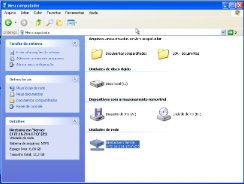
\includegraphics[width=0.7 \textwidth]{figuras/mapeamento}
   	\caption{Tela de um mapeamento}
    \label{mapeamento}
\end{figure}

\section{Compartilhamento de Impressoras}

O compartilhamento de impressora é a publicação das impressoras instaladas no servidor para que outras máquinas que estão na rede possam acessar e imprimir sem precisar da conexão local na impressora.

Para compartilhar as impressoras com o Samba 3 deve-se adicionar na seção [global] as variáveis contidas no Quadro \ref{smb_print}\\

\begin{lstlisting}[caption=Variáveis para permitir impressão em impressoras compartilhadas,label={smb_print}]	
[global]

printing = cups

load printers = yes	
\end{lstlisting}

\begin{itemize}
	\item \textbf{printing} - Define qual o programa será utilizado para gerenciar as impressões 
	\item \textbf{load printers} - Carrega as impressoras
\end{itemize}

O Samba 3 utiliza o cups que é o gerenciador de impressoras mais comum para o Linux.

\begin{enumerate}
	\item \textbf{\#smbd -b $|$ grep CUPS} - Para saber se o pacote Samba 3 instalado é compatível com o CUPS. A saída deve ser algo como ``HAVE CUPS"
\end{enumerate}

Caso o cups não esteja instalado.

\begin{enumerate}
	\item \textbf{\#apt-get install cups} - Instala todos os pacotes necessários para o funcionamento do cups.
	\item \textbf{\$ firefox localhost:631} - Interface gráfica para gerenciar as impressoras. Figura \ref{cups}.
	\item \textbf{\# /etc/init.d/cupsys restart} - Reinicia o serviço do cups
\end{enumerate}

\begin{figure}[ht]
   	\centering
    \scalebox{1}{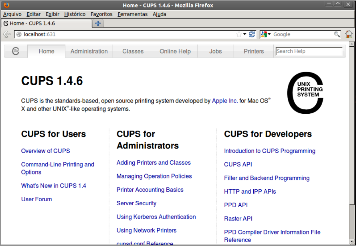
\includegraphics{figuras/cups}}
   	\caption{Tela do CUPS pelo Browser}
    \label{cups}
\end{figure}

Para habilitando o compartilhamento de impressora. Tem que adicionar as variáveis contidas no Quadro \ref{smb_printer}\\

\begin{lstlisting}[caption=Variáveis para compartilhar impressoras,label={smb_printer}]	
[printers]

print ok = yes

guest ok = yes

path = /var/spool/samba

browseable = yes	
\end{lstlisting}

\begin{itemize}
	\item \textbf{path} - Esse caminho é onde ficarão os spools de impressão. Esse diretório é criado automaticamente pelo Samba 3 e deve ter a permissão 777.
	\begin{enumerate}
		\item \textbf{chmod 777 -R /var/spool/samba}
	\end{enumerate}
\end{itemize}

Dessa forma ao acessar o servidor irão aparecer todas as impressoras instaladas.

\section{Instalação automática dos driver da impressora}

Para conectar-se a uma impressora compartilhada é necessário a instalação dos drivers da mesma. 

Um problema é como esses drivers são armazenados e instalados, já que uma das formas de instalar esses drivers é ir até o computador com o instalador em cd ou pen-drive e realizar a instalação manualmente, porém em uma grande rede se perde muito tempo com a locomoção e instalação. A solução desse problema é a instalação automática dos drivers, e com a utilização do Samba 3 os drivers serão instalados assim que o usuário tentar conectar a impressora.

Adiciona no [global]

\begin{itemize}
	\item \textbf{enable privileges = yes} - Permite privilégios a usuários
\end{itemize}

Criar um compartilhamento não visível onde ficará os drivers das impressoras. Conforme mostrado no Quadro \ref{smb_print_driver}\\

\begin{lstlisting}[caption=Variáveis para compartilhamento onde deverão ficar os \textit{drivers} das impressoras,label={smb_print_driver}]	
[print$]

path = /var/lib/samba/printers

read only = yes

write list = root

inherit permissions = yes	
\end{lstlisting}

\begin{itemize}
	\item \textbf{path} - Local onde os drivers serão instalados
	\item \textbf{write list} - Usuários ou grupos que terão permissão de escrita
	\item \textbf{inherit permissions} - Se os arquivos irão herdar as permissões da pasta.
\end{itemize}

Se o caminho apontado pelo path não existir ele terá que ser criado com as permissões necessárias.

\begin{enumerate}
	\item \textbf{\# mkdir -p /var/lib/samba/printers}
	
	\item \textbf{\# cd /var/lib/samba/printers}
	\item \textbf{\# mkdir WIN40 W32X86} - Essas pastas são os locais onde ficarão os drivers das impressoras, o WIN40 para sistemas Windows 95/98/ME e o W32X86 Windows NT/2000/XP.
	\item \textbf{\# chown dtic WIN40 W32X86} - Muda o proprietário da pasta para que o usuário dtic tenha permissão para escrever no diretório.
	\item \textbf{\# smbpasswd -a dtic} - Cadastra o usuário no Samba 3. O usuário dtic já estava devidamente criado localmente no Linux.
	\item \textbf{\# chmod 2775 WIN40 W32X86} - Permissões especiais para instalar os drivers nos usuários.
	\item \textbf{\# net -S localhost -U root -W NOME\_DO\_SERVIDOR  rpc rights grant ``NOME DO SERVIDOR$\backslash$dtic" SePrintOperatorPrivilege} - Irá definir que o usuário dtic terá todas os privilégios necessários para gerenciar as impressoras.
\end{enumerate}

Com as permissões, usuários e impressoras configuradas, os \textit{drivers} tem que ser passados para o servidor. Para tal, é necessária a utilização de uma máquina cliente com Windows instalado. Ela se conectará ao servidor que está compartilhando as impressoras, e através da senha de root desse servidor, irá passar os \textit{drivers} através da rede. A sequência de figuras a seguir ilustra o passo-a-passo para a adição desses \textit{drivers}.

\begin{enumerate}
	\item \textbf{Acesse a maquina com um usuário local} - Figura \ref{login_windows_local}
		\begin{figure}[ht]
		   	\centering
		    \scalebox{1}{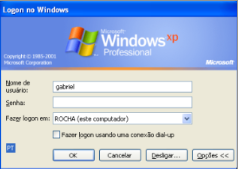
\includegraphics{figuras/login_windows_local}}
		   	\caption{Tela do Login no Windows localmente}
		    \label{login_windows_local}
		\end{figure}
		
	\item \textbf{Informe o endereço do servidor} - Figura \ref{server_ip}	
	\begin{figure}[ht]
	   	\centering
	    \scalebox{1}{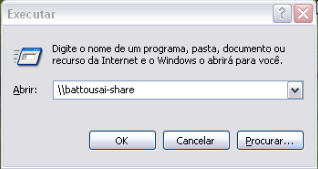
\includegraphics{figuras/server_ip}}
	   	\caption{IP do servidor de compartilhamento}
	    \label{server_ip}
	\end{figure}
		
\pagebreak
	
	\item \textbf{Informe o usuario root e sua senha.}	
	
	\item \textbf{Acesse a pasta ``Impressoras e aparelhos de fax"} - Figura \ref{impressora_aparelho_fax}
	\begin{figure}[ht]
	   	\centering
	    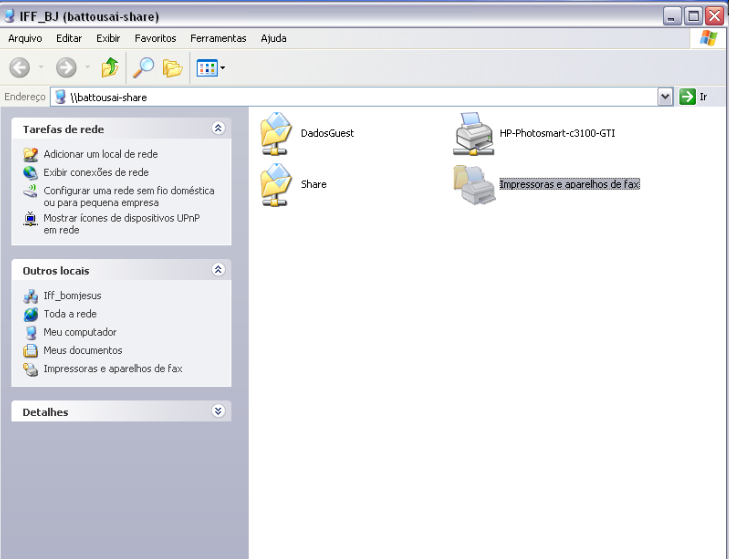
\includegraphics[width=0.7 \textwidth]{figuras/impressora_aparelho_fax}
	   	\caption{Impressoras e aparelhos de fax compartilhados}
	    \label{impressora_aparelho_fax}
	\end{figure}

%	\pagebreak

	\item \textbf{Clique na opção Arquivos -$>$ Propriedade do servidor.}
	
%	\pagebreak
	
 	\item \textbf{Aba Driver -$>$ Adicionar} - Figura \ref{adicionar_driver}
	\begin{figure}[ht]
	   	\centering
	    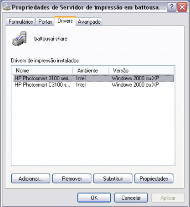
\includegraphics[width=0.7 \textwidth]{figuras/adicionar_driver}
	   	\caption{Adicionar driver ao servidor de impressão}
	    \label{adicionar_driver}
	\end{figure}
	
	\pagebreak
	
	\item \textbf{Selecione o driver da impressora que deve ser copiado para o servidor} - Figura \ref{selecionar_driver}
	\begin{figure}[ht]
	   	\centering
	     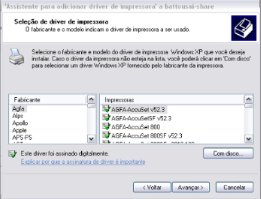
\includegraphics[width=0.7 \textwidth]{figuras/selecionar_driver}
	   	\caption{Selecionar o driver que será copiado para o servidor de impressão}
	    \label{selecionar_driver}
	\end{figure}
	
	
	\item \textbf{Selecione os sistemas operacionais dos \textit{drivers} que serão instalados, e avance até concluir o assistente.} - Figura \ref{selecionar_so}
	\begin{figure}[ht]
	   	\centering
	     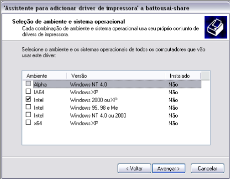
\includegraphics[width=0.7 \textwidth]{figuras/selecionar_so}
	   	\caption{Selecionar os Sistemas Operacional que o driver será compatível}
	    \label{selecionar_so}
	\end{figure}
	
	\pagebreak
	
	\item \textbf{Ao sair do assistente, clique com o botão direito na impressora desejada, e clique em Propriedades.} - Figura \ref{propriedade_impressora}
	\begin{figure}[ht]
	   	\centering
	     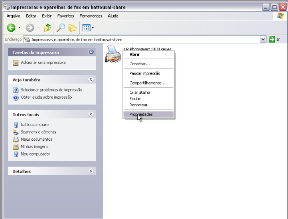
\includegraphics[width=0.7 \textwidth]{figuras/propriedade_impressora}
	   	\caption{Propriedade da impressora do compartilhamento}
	    \label{propriedade_impressora}
	\end{figure}

	
	\item \textbf{Na caixa de mensagem que irá aparecer, selecione a opção ``NÃO", pois caso selecione o sim o \textit{driver} será instalado somente na maquina local.} - Figura \ref{opcao_nao}
	\begin{figure}[ht]
	   	\centering
	     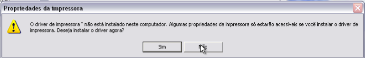
\includegraphics[width=0.7 \textwidth]{figuras/opcao_nao}
	   	\caption{Opção para não instalar o driver naquele momento}
	    \label{opcao_nao}
	\end{figure}
	
	\item \textbf{Na guia avançado, selecione o \textit{drive} que será vinculado a impressora e clique em OK.} - Figura \ref{aba_avancado}
	\begin{figure}[ht]
	   	\centering
	     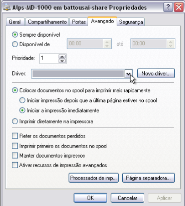
\includegraphics[width=0.7 \textwidth]{figuras/aba_avancado}
	   	\caption{Aba onde será feito o link da impressora com o driver}
	    \label{aba_avancado}
	\end{figure}
	
		\pagebreak
		
	\item \textbf{Após esses passos, o \textit{driver} da impressora já estará instalado no servidor de impressão. A partir desse momento, para instalar essa impressora, basta logar com o usuário do domínio no qual a impressora está compartilhada.} - Figura \ref{login_dominio}
	\begin{figure}[ht]
	   	\centering
	     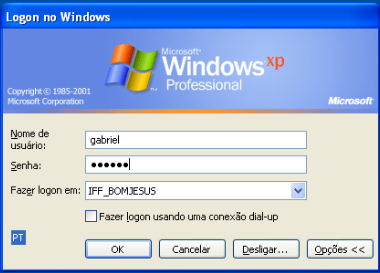
\includegraphics[width=0.7 \textwidth]{figuras/login_dominio}
	   	\caption{Logar no domínio}
	    \label{login_dominio}
	\end{figure}
	
	% \pagebreak
	
	\item \textbf{Acesse o servidor, conforme passo 2, e selecione a impressora que deseja mapear.} - Figura \ref{selecionar_impressora_servidor}
	\begin{figure}[ht]
	   	\centering
	     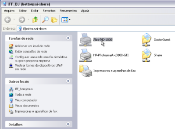
\includegraphics[width=0.7 \textwidth]{figuras/selecionar_impressora_servidor}
	   	\caption{Selecionar a impressora que será mapeado no usuário logado}
	    \label{selecionar_impressora_servidor}
	\end{figure}
	
%	\pagebreak
	
	\item \textbf{Após esses passos, a impressora será instalada automaticamente no computador cliente sem a necessidade de \textit{drivers} adicionais, pois estes foram disponibilizados automaticamente pelo servidor através da rede.} - Figura \ref{impressora_compartilhada}
	\begin{figure}[ht]
	   	\centering
	     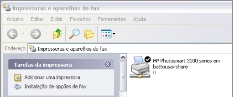
\includegraphics[width=0.7 \textwidth]{figuras/impressora_compartilhada}
	   	\caption{Impressora instalada no usuário}
	    \label{impressora_compartilhada}
	\end{figure}
	
\end{enumerate}

%\pagebreak

\section{Ingressando o Windows XP no Domínio}

Para ingressar um computador Windows no domínio através do Samba 3 é necessário que primeiramente ele esteja devidamente cadastrado no servidor Samba 3. O Windows deve estar com os drivers de rede instalados e respondendo na rede.
Para ingressar o Windows XP no domínio deve-se realizar os seguintes passos:

\begin{enumerate}
	\item {Realize logon no Windows com uma conta que possua privilégios administrativos. - Figura \ref{logon_local_adm}}
	\begin{figure}[ht]
   			\centering
   			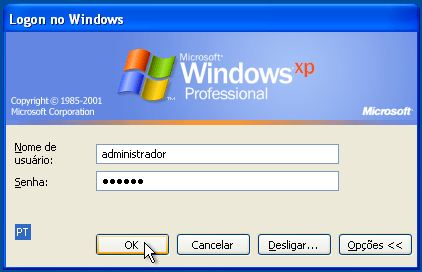
\includegraphics[width=0.7 \textwidth]{figuras/logon_local_adm}
   			\caption{Tela de logon local}
    		\label{logon_local_adm}
	\end{figure}

	\item {Após o logon, deve-se abrir o programa Executar no menu Iniciar e acessar as Propriedades do Sistema através do comando ``sysdm.cpl".}

	\item {Acessar a aba ``Nome do Computador". Deve-se clicar no botão ``Alterar". - Figura \ref{alterar_nome_micro}}

		\begin{figure}[ht]
	   			\centering
	   		 	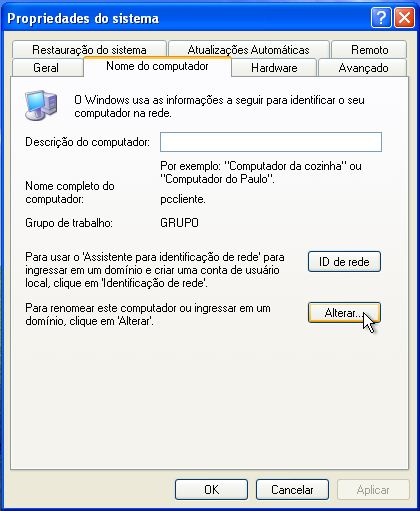
\includegraphics[width=0.7 \textwidth]{figuras/alterar_nome_micro}
	   			\caption{Alterando nome do micro}
	    		\label{alterar_nome_micro}
		\end{figure}
		 
		\pagebreak 

	\item {No menu de ``Alterações de nome do computador", certifique-se de que o nome definido para o computador é o mesmo que foi cadastrado no servidor Samba 3. No campo ``Membro de", selecione a opção ``Domínio" e digite o nome do domínio definido na sessão [global] do Samba 3 e depois clique em OK. - Figura \ref{incluir_dominio}} 
			\begin{figure}[ht]
		   			\centering
		   		 	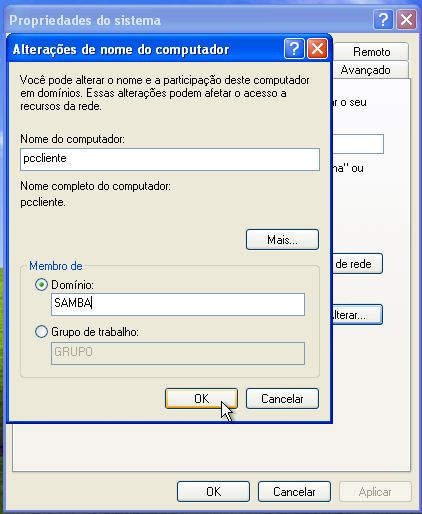
\includegraphics[width=0.7 \textwidth]{figuras/incluir_dominio}
		   			\caption{Incluir micro no domínio}
		    		\label{incluir_dominio}
			\end{figure}
	 
	%\pagebreak
	
	\item {Insira a senha de administrador do servidor para o micro ingressar no domínio. E aguarde a mensagem de confirmação.} 
	
	\item {Reinicie o micro quando for solicitado pelo sistema.}

	\item {Após inicialização o micro, selecione o domínio para realizar o logon e entre com um usuário e senha que esteja cadastrados previamente no servidor. - Figura \ref{logon}}
	\begin{figure}[ht]
			\centering
	 		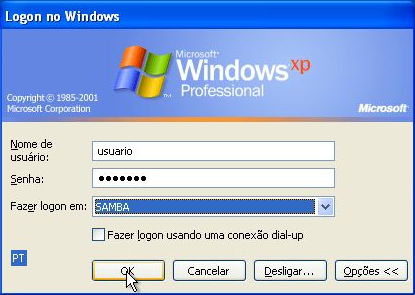
\includegraphics[width=0.7 \textwidth]{figuras/logon}
			\caption{Efetuando logon no domínio}
			\label{logon}
	\end{figure}

\end{enumerate}

%\pagebreak

\section{Ingressando o Linux no Domínio}

Para ingressar um computador Linux no domínio é necessário que primeiramente ele esteja devidamente cadastrado no servidor Samba 3. Para o Linux realize login no servidor PDC é necessário a instalação de três pacotes essenciais. São eles o Samba, o Winbind e os módulos do PAM (libpam-modules).

A instalação desses pacotes na distribuição Ubuntu pode ser realizada através dos comando:

\begin{enumerate}
	\item \textbf{\#apt-get update} - Atualiza a base de dados do repositório.
	\item \textbf{\#apt-get install samba winbind libpam-modules} - Realiza a instalação dos pacotes Samba, Winbind e módulos do PAM.
\end{enumerate}

Após a instalação é necessário realizar a configuração do micro para que possa fazer login no domínio. Começando pela configuração do Samba através do arquivo de configuração \textbf{/etc/samba/smb.conf}, que deve ser editado para que a seção [global] fique conforme o Quadro \ref{login_global_smb}. Pode-se optar por adicionar essa configuração à configuração existente, ou pode manter apenas essa configuração básica:\\

\begin{lstlisting}[caption=Arquivo smb.conf com as variáveis necessárias para fazer login em um domínio,label={login_global_smb}]	
[global]

workgroup = Dominio

netbios name = cliente1

winbind use default domain = yes

obey pam restrictions = yes

security = domain

encrypt passwords = true

wins server = 192.168.1.1

winbind uid = 10000-20000

winbind gid = 10000-20000

template shell = /bin/bash

template homedir = /home/\%U
\end{lstlisting}

Explicação de algumas variáveis importantes:
\begin{itemize}
	\item \textbf{workgroup} - Nome do domínio configurado no servidor Samba 3.
	\item \textbf{netbios name} - Nome do computador cliente (/etc/hostname), que deve estar cadastrado no servidor.
	\item \textbf{wins server} - Ip do servidor PDC Samba 3.
\end{itemize}

Editado o arquivo \textbf{/etc/samba/smb.conf}, deve-se testar o arquivo de configuração para verificação de erros através do comando \textbf{\#testparm}.
Após a configuração do Samba, deve-se configurar o arquivo \textit{Network Services Switch} (\textbf{/etc/nsswitch.conf}), que determina a ordem das buscas quando uma informação é solicitada. Esse arquivo deve ter as seguintes linhas do Quadro \ref{nsswitch_login} alteradas:\\

\begin{lstlisting}[caption=Arquivo nsswitch.conf,label={nsswitch_login}]	
passwd: compat winbind

group: compat winbind

shadow: compat winbind	
\end{lstlisting}

Foi incluído o \textbf{winbind} nas variáveis de busca \textbf{passwd}, \textbf{group} e \textbf{shadow} para que esses valores sejam buscados no servidor Samba 3.

Depois de concluídas as configurações, é necessário reiniciar o Samba e o Winbind.

\begin{enumerate}
	\item \#service winbind restart
	\item \#service smbd restart
	\item \#service nmbd restart	
\end{enumerate}


Para testar a configuração realizada deve-se fazer o ingresso no domínio conforme abaixo. Será retornada uma mensagem de sucesso como a do Quadro \ref{result_join}.\\

\begin{itemize}
	\item \#net rpc join member -U root
\end{itemize}

\begin{lstlisting}[caption=Resultado quando a máquina é adicionada com sucesso no domínio,label={result_join}]	
Password:

Joined domain DOMINIO.
\end{lstlisting}

Observação: A senha solicitada é a senha de root do servidor PDC, cadastrada no Samba.

Os arquivos a serem alterados em seguida serão as os arquivos de políticas de funcionamento do PAM. Essas políticas se encontram no diretório \textbf{/etc/pam.d}, onde está contido os arquivos de configuração pra cada serviço que utilize os módulos de autenticação do PAM. O nome de um arquivo nesse diretório indica a qual serviço o arquivo de configuração se refere (portanto o arquivo \textbf{/etc/pam.d/login} fará referência ao serviço de \textit{LOGIN} do Linux).
Para definir políticas de autenticação a um serviço, deve-se acessar o arquivo do serviço desejado acrescentar as configurações desejadas seguindo a seguinte sintaxe do Quadro \ref{pam.d}:\\

\begin{lstlisting}[caption=Exemplo de configuração do /etc/pam.d/login,label={pam.d}]
auth	required	pam_nologin.so	no_warn
\end{lstlisting}

Cada linha de configuração é formada por 4 campos. No exemplo temos os 4 campos na seguinte ordem: Nome instalação, tag de controle, nome do módulo, e argumentos do módulo. Campos adicionais serão interpretados como argumentos do módulo.

Após o teste de ingresso no domínio é necessário configurar o sistema de autenticação PAM para busca os logins no servidor. Para isso é necessário modificar os arquivos \textbf{/etc/pam.d/login} e \textbf{/etc/pam.d/gdm}. O arquivo \textbf{/etc/pam.d/login} é responsável pelas configurações de autenticação de usuários no sistema, enquanto o arquivo \textbf{/etc/pam.d/gdm} é responsável pelas configurações de autenticação na interface de login do gnome.
No arquivo \textbf{/etc/pam.d/login}, deve-se adicionar as linhas do Quadro \ref{pam_login} no inicio do arquivo:\\

\begin{lstlisting}[caption=Linhas do arquivo /etc/pam.d/login,label={pam_login}]
session required pam_mkhomedir.so skel=/etc/skel umask=0022

session optional pam_mount.so

auth sufficient pam_winbind.so

account sufficient pam_winbind.so

session required pam_winbind.so
\end{lstlisting}

No arquivo \textbf{/etc/pam.d/gdm} deve-se comentar todo o seu conteúdo e adicionar as linhas contidas no Quadro \ref{pam_gdm} ao inicio do arquivo:\\

\pagebreak

\begin{lstlisting}[caption=Arquivo /etc/pam.d/gdm,label={pam_gdm}]	
auth required /lib/security/pam_securetty.so

auth required /lib/security/pam_nologin.so

auth sufficient /lib/security/pam_winbind.so

auth required /lib/security/pam_pwdb.so use_first_pass shadow nullok

account required /lib/security/pam_winbind.so

session required /lib/security/pam_mkhomedir.so skel=/etc/skel umask=0022
\end{lstlisting}

As configurações acima fazem com que a tela de login exiba os usuários disponíveis no servidor para ingresso diretamente no domínio sem que haja autenticação local. Para as configurações acima funcionarem corretamente, a opção de Login Automático não pode estar ativada no computador.